\section{Validating Physics-Informed Neural Network (PINN) code}
\par{}
Validating the enhanced PINN code was done with two chosen problems. First one
is to approximate the same parabola profile but with equation \(y=x^2\) instead
of y-data, and the second one is to model the fluid velocity decay profile due
to fluid viscosity, which involves differential equation. \\

\subsection{Parabola profile with equation}
\par{}
The problem is similar to the one used for validating the neural network code
earlier, except the fact that, the y-data is made unavailable and the
governing equation \(y=x^2\) is given instead. The residual of the equation
will be given to the loss function which has to be minimized for training the
model. The network architecture is given in \cref{parabola_PINN_network}.
And the estimated vs expected results graph is given in \cref{parabola_PINN_result}.\\

\begin{figure}
   \center
    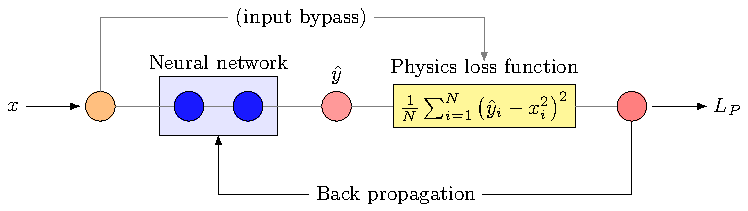
\includegraphics[scale=1]{supportingFiles/01_schematics/04_parabola_PINN_network/parabola_PINN.pdf}
    \caption{PINN network schematic for parabola problem}
    \label{parabola_PINN_network}
\end{figure}

\begin{figure}
   \center
    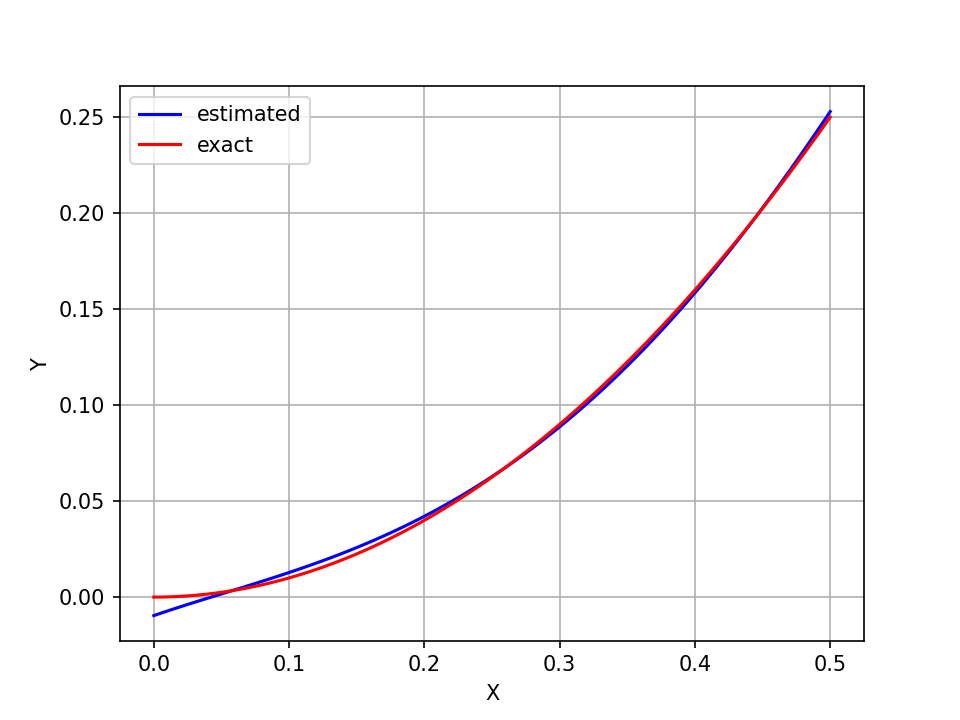
\includegraphics[scale=0.7]{supportingFiles/02_results/04_parabola_PINN/estimation.png}
    \caption{Parabola estimated vs exact result using PINN}
    \label{parabola_PINN_result}
\end{figure}

\subsection{Exponential velocity decay due to fluid viscosity}
\par{}
Given a point in a free fluid flow, the velocity of fluid particles will decay
at the point due to the resistance termed as fluid viscosity. This decay
will be in exponential form and is governed by \cref{velocity_decay_equation},
which was already discussed partially in the derivative validation section.

\begin{align}
    \frac{d V}{d t} = -k V \label{velocity_decay_equation}
\end{align}

Here, \(k\) is a constant denoting fluid viscosity.
The equation is of autonomous form and has analytical solution given as below.

\begin{align*}
    V = V_0 e^{-k t}
\end{align*}

\(V_0\) is the initial velocity of the fluid flow. Schematic of the PINN used
for the problem is given in \cref{velocity_decay_PINN_schematic}. Here, the
network has two hidden layers with 3 and 2 neurons respectively, and an
output layer with 1 neuron. \(tanh()\) activation function was used in all
the layers.\\

\begin{figure}
   \center
    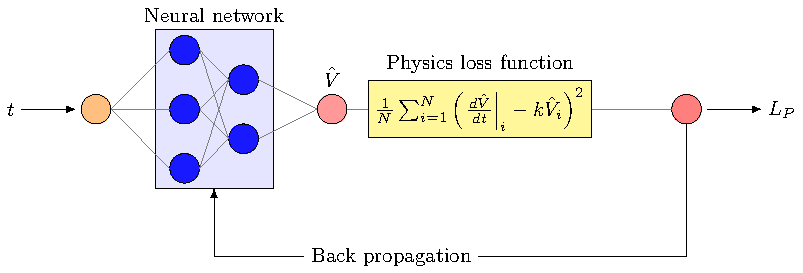
\includegraphics[scale=1]{supportingFiles/01_schematics/05_velocity_PINN_network/velocity_PINN.pdf}
    \caption{Velocity decay problem PINN schematic}
    \label{velocity_decay_PINN_schematic}
\end{figure}

\par{}
The loss function of this network is made in two parts, the first part will enforce
the initial condition of velocity and will be made active only at the starting
of time data, it is given as below.
\begin{align}
    L_{IC} = \left.\left(\hat{V}_i - V_i\right)^2\right|_{t=0, i=0} \label{IC_eqn}
\end{align}

The second part will contain the governing equation constraint and that will be
executed for all timesteps. The equation is as given below.

\begin{align}
    L_{ODE} = \frac{1}{N}\sum_{i=0}^{N}\left(\left.\frac{d\hat{V}}{dt}\right\vert_i - k\hat{V}_i\right)^2 \label{ODE_eqn}
\end{align}

So, the total loss function for the network will be sum of \cref{IC_eqn,ODE_eqn},
as given below.
\begin{align}
    L = L_{IC}+L_{ODE} =  \left.\left(\hat{V}_i - V_i\right)^2\right|_{t=0, i=0}+\frac{1}{N}\sum_{i=0}^{N}\left(\left.\frac{d\hat{V}}{dt}\right\vert_i - k\hat{V}_i\right)^2 \label{velocity_decay_LF}
\end{align}

Actually, to increase the weightage of initial condition as it is active only
in a part of the back propagation, a factor of 10 was multiplied to its compontent
and the final loss equation is given as below.
\begin{align}
    L = L_{IC} \times 10+L_{ODE} \label{velocity_decay_PINN_LF}
\end{align}

\par{}
The model was trained successfully, and the estimated results of velocity
profile and the derivative computation were given in
\cref{velocity_decay_PINN_results}.  It was found that the derivative estimated
was accurate than the one shown for the validation. This is because the network
that learns a function through physics constraints learn better than the
network that maps the same function through data. \\

\begin{figure}
    \begin{subfigure}{0.5\linewidth}
       \center
        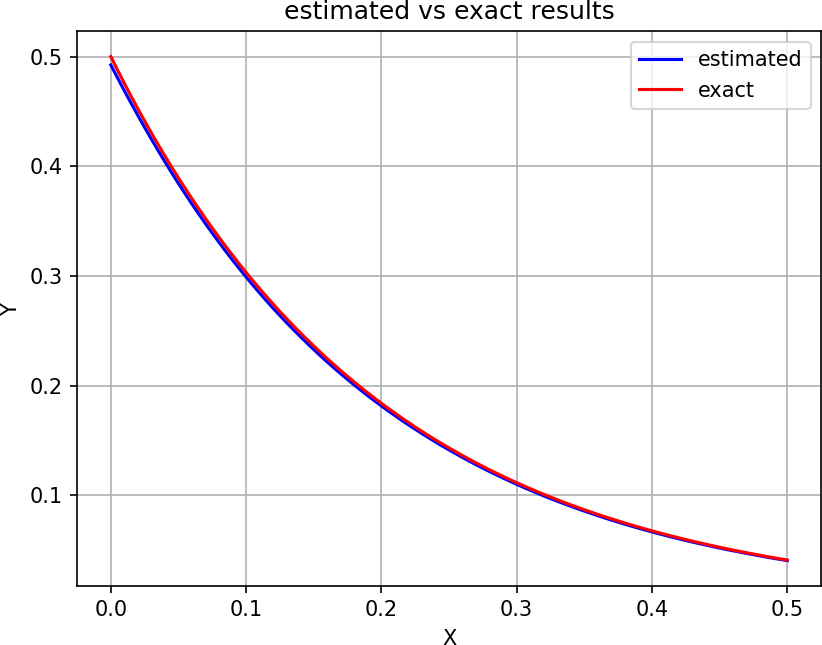
\includegraphics[scale=0.5]{supportingFiles/02_results/05_velocity_decay/estimated_output.png}
        \caption{Estimated vs expected velocity decay profile, (here X = t, Y = V)}
        \label{}
    \end{subfigure}
    \hfill
    \begin{subfigure}{0.5\linewidth}
       \center
        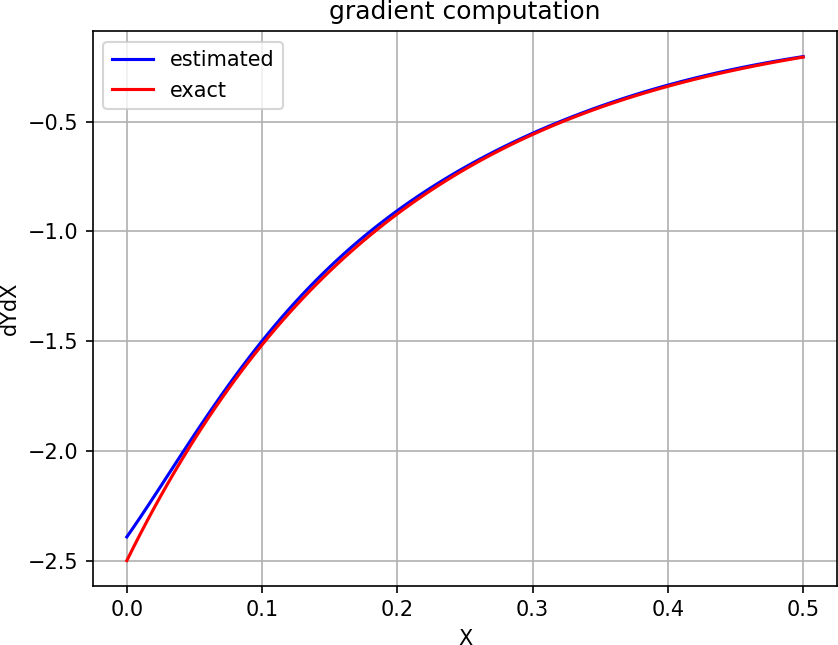
\includegraphics[scale=0.5]{supportingFiles/02_results/05_velocity_decay/gradient_computation.png}
        \caption{Estimated vs expected gradient profile, (here X = t, Y = V)}
        \label{}
    \end{subfigure}
    \caption{Exponential velocity decay due to fluid viscosity problem solution using PINNs}
    \label{velocity_decay_PINN_results}
\end{figure}

\par{}
The error percentage graph for the estimated vs expected velocity profiles
was given in \cref{velocity_PINN_EP_graph}. The error percentage were in the
order of 1-2\%, hence this validates the PINN code developed.

\begin{figure}
   \center
    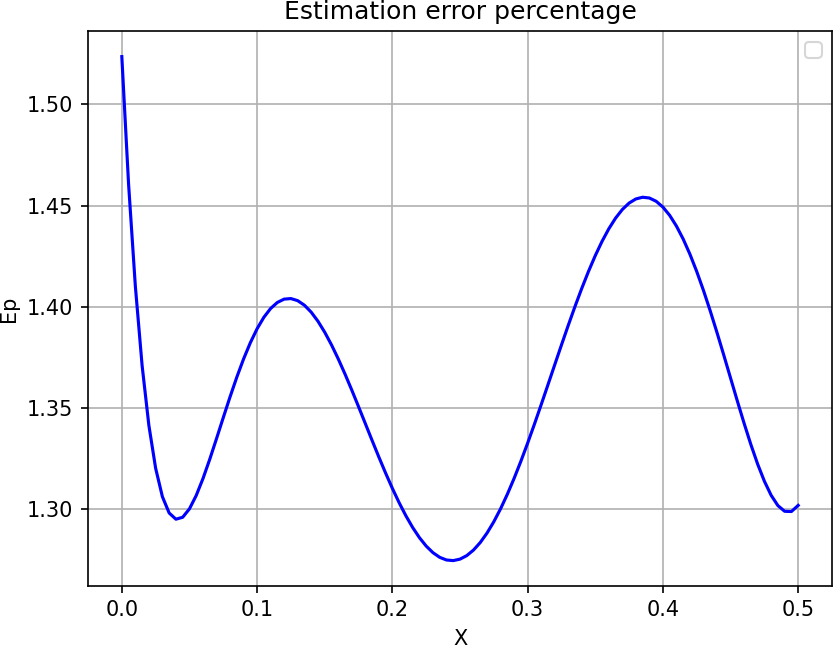
\includegraphics[scale=0.7]{supportingFiles/02_results/05_velocity_decay/error_percentage.png}
    \caption{Error percentage of estimated vs expected velocity profiles}
    \label{velocity_PINN_EP_graph}
\end{figure}
